\chapter{Experiments}
\label{chap:design}

\paragraph{Origin of the experiments}
At the beginning of our research into the performance and scalability of common Kubernetes and Open vSwitch configurations, we did not know which part of the networking stack will lead to interesting results and where to focus on. So we started practically experimenting with packet handling and always continued based on our previous results. In the end, our exploration led us to focus on upcall handling and flow rule management.

As we showed in \cref{chap:refs}, OVS inserts flow rules into datapaths on demand after upcalls. Therefore packets generating upcalls are more expensive to process than the other packets. We tried to create a network traffic, which would reliably generate upcalls to study the behavior of OVS under stress. This chapter describes the details of our research.

\paragraph{The experiments}
We split our research into the following parts:

\begin{enumerate}
    \item We investigated flow rule handling in OVS. If we sent the same packet twice, the second will always hit a rule in the datapath and it will not generate an upcall. Except for cases, when the flow rule is already removed. When does that happen? When are flow rules removed from the datapaths? We investigated this in \cref{design:flow-eviction}.

    \item What is the cost of an upcall? How much slower is the slow path compared to the fast path? Can we infer whether upcall-only traffic will be a significant performance problem? (\cref{design:upcall-cost})

    \item Once we knew the flow rule timeout, we could investigate packet types generating upcalls. Which packet header values lead to a generation of new flow rules? (\cref{design:upcall-generators})

    \item The last and most significant part - what is the impact of artificial upcall-only traffic on the performance of the whole system? We investigated this in \cref{design:upcall-impact}.
\end{enumerate}

Most of the questions above can be approached using both static and dynamic analysis (analyzing the source code or analyzing the behavior of a running system). At the beginning of our investigation, we were not familiar with the relevant code and we also did not know what exactly to focus on, so we always started with a dynamic analysis, because it allowed us to observe the behavior of the whole networking stack. After the initial practical experiment, we searched for the code causing the observed behavior.

In the following sections, we discuss the design of our experiments and their results. Every following section corresponds to one of the investigation parts mentioned above.

\section{Flow eviction timeout}
\label{design:flow-eviction}

We can observe an effect of an upcall using the \ident{ping} tool. The first packet has higher latency than the rest of the ICMP packets because it generates an upcall and a new datapath flow rule (can be verified by \ident{ovs-dpctl dump-flows}).

\vspace{0.5cm}
\begin{lstlisting}[caption=Output of the \ident{ping} command in the virtualized environment, captionpos=b, basicstyle=\ttfamily\scriptsize]
[root@kb2 ~]# ping -c 5 kb3
PING kb3 (192.168.1.223) 56(84) bytes of data.
64 bytes from kb3 (192.168.1.223): icmp_seq=1 ttl=64 time=1.19 ms
64 bytes from kb3 (192.168.1.223): icmp_seq=2 ttl=64 time=0.404 ms
64 bytes from kb3 (192.168.1.223): icmp_seq=3 ttl=64 time=0.365 ms
64 bytes from kb3 (192.168.1.223): icmp_seq=4 ttl=64 time=0.424 ms
64 bytes from kb3 (192.168.1.223): icmp_seq=5 ttl=64 time=0.304 ms

--- kb3 ping statistics ---
5 packets transmitted, 5 received, 0% packet loss, time 4062ms
rtt min/avg/max/mdev = 0.304/0.536/1.185/0.326 ms
\end{lstlisting}

To repeat the observation, we must not send similar ICMP packets for several seconds. The higher latency is measurable only when we wait. This behavior can be explained by a flow rule eviction timeout that removes the rule from the datapath's forwarding table.

Assuming the timeout stays constant, we can measure it by varying the interval between ICMP packets. The dependency between the measured latency and the time delay should be constant except for one sharp increase in latency when the delays get longer than the timeout.

\paragraph{Our experiment}
We experimented in the following way:

\begin{enumerate}
    \item Generate a random number $D$ in the interval $\interval{8}{12}$
    \item sleep for $D$ seconds
    \item run \ident{ping -c 3 -i 0.01 192.168.1.221}
    \item log $D$ and both round trip times
    \item go to step 1 until we have enough samples
\end{enumerate}

We chose the interval based on non-rigorous preliminary experiments. After plotting RTT's dependence on the delay $D$, we expect to see:

\begin{itemize}
    \item The first RTT data points will form a line with a sharp increase at a value of $D$ corresponding to the eviction timeout

    \item The second RTT data points will form only a single horizontal line.

    \item The third ping will have the same results as the second.
\end{itemize}

The practical nature of this experiment allows us to check OVS's configuration even on systems where we do not have privileges to access OVS directly.

\subsection{Results}
\label{res:eviction-timeout}

\begin{figure}
    \centering
    \includegraphics[width=.9\linewidth]{img/randomized_eviction_timeout.png}
    \caption{Results of the eviction timeout experiment}
    \label{fig:plot-eviction-timeout}
\end{figure}

\paragraph{The eviction timeout} The measured latencies of the experiment (\cref{fig:plot-eviction-timeout}) show the flow rule eviction taking effect about $10$ seconds after the last datapath rule installation. The observed value is not exact, but it is probably reasonable to assume the developers chose a nice-looking number. We hypothesize that the noise in the location of the increase is introduced mainly by infrequent eviction checks.

Following these experimental findings, we searched the source code and it specifies exactly $10$ seconds as the default eviction timeout. The experimental findings are consistent with the source code. The default rule timeout is defined in the file \ident{ofproto/ofproto.h} as:
\begin{verbatim}
#define OFPROTO_MAX_IDLE_DEFAULT 10000 /* ms */
\end{verbatim}

The file \ident{ofproto/ofproto-dpif-upcall.c} contains the code enforcing the timeout in the function \ident{revalidate()}:

\begin{verbatim}
if (kill_them_all || (used && used < now - max_idle)) {
    result = UKEY_DELETE;
}
\end{verbatim}

The eviction is handled by the revalidator threads, which run periodically roughly every 500ms. This confirms our hypothesis about the $~500$ms spread of the observable timeout effect.

\begin{verbatim}
// in file ofproto/ofproto.h:321
#define OFPROTO_MAX_REVALIDATOR_DEFAULT 500 /* ms */

// in the ofproto/ofproto_dpif_upcall.c:1052
// in function udpif_revalidator()
poll_timer_wait_until(start_time + MIN(ofproto_max_idle,
                                    ofproto_max_revalidator));
\end{verbatim}

\paragraph{Difference in latency below timeout}
\Cref{fig:plot-eviction-timeout} shows a difference between round trip times for the first and second packet even for delays shorter than the eviction timeout. The difference is small, so we assume that this can be caused by CPU caches. We did not investigate this further.

\paragraph{Increase in round trip time of the second ping}
\Cref{fig:plot-eviction-timeout} also shows an increased latency for the second ping after the eviction timeout. We hypothesize that it could be caused by the fixed size flow lookup cache described in \cref{subsec:matching-algo}. The upcall installs the new flow, but the lookup cache is filled only after the first use (i.e. the second packet of the flow, the second ICMP ping). In other words, if we would send multiple packets, their journey through the \ident{openvswitch} module would be as follows:

\begin{enumerate}
    \item A cache miss, followed by a flow table miss. Leads to an upcall and a new flow rule.
    \item A cache miss, which requires a full flow table scan. The cache is filled.
    \item Cache hit.
    \item All consecutive packets hit the cache unless the cache entry is somehow overwritten.
\end{enumerate}

The third RTT measurement behaves as expected by our hypothesis. We shortly experimented with even more consecutive measurements and they were all the same.


\section{Cost of an upcall}
\label{design:upcall-cost}

Eelco Chaudron investigated the cost of an upcall in OVS \cite{UpcallCost} using eBPF probes in the Linux kernel. His experiments show that processing a packet through the slow path can take anywhere between \qty{150}{\us} and \qty{10}{\ms} extra compared to the fast path. However, as we saw in the previous section, upcalls have visible effects outside of the kernel and we can measure them directly.

The unchanged experiment devised in the previous section provides us with a direct measurement of the observable upcall effect. The difference between the first packet RTT and the second packet RTT should correspond to how much time an upcall costs.

% While this measurement methodology leads to less precise results than when directly measuring the in-kernel execution time using eBPF, we can use it to measure the upcall cost without special privileges on publicly deployed cloud hosting services.\todo{má smysl tohle zmiňovat, když to nezkusím? Napsal jsem do MetaCentra a domluvili jsme se, ze se mi ozvou. Ale zatim nic.}

This experiment assumes that ICMP packet processing in OVS is the same as for all other types of packets. We believe this is most likely correct because OVS generates datapath flow rules for handling ICMP packets the same as it does for all other packets. Also, we did not find any evidence of ICMP packets being handled specially.

\subsection{Results}
\label{res:upcall-cost}

\paragraph{Upcall processing cost}
As discussed in \cref{chap:design}, the round trip time increase can be attributed to the cost of upcall processing. In the previous section, we noticed an increased latency with the second RTT measurement, possibly a cache miss in the kernel datapath.  We can estimate the cost of an upcall using this data. We calculated the difference between the first and the second ping measurements and assume the result is the lower bound for the upcall cost. Either our hypothesis about the cache miss is correct. Then the difference would be exactly the time spent processing the upcall. Or, we are wrong and the higher second ping latencies are caused by some additional factor that is not normally present. In that case, the upcall cost would be certainly equal to or higher than our result. For our calculation, we used only latency measurements with the delay since the previous measurement larger than $10.5$ seconds.

% QT_QPA_PLATFORM=xcb python postprocessing/randomized_eviction_timeout.py results/randomized_eviction_timeout/*.csv
\begin{table}[h!]
    \begin{center}
        \caption{Statistics of measured round trip times when the interval > 10.5 seconds}
        \label{tab:upcall-cost}
        \begin{tabular}{r|S[table-format=4.2]S[table-format=4.2]S[table-format=4.2]}
            & \textbf{First ping RTT} & \textbf{Second ping RTT} & \textbf{Difference} \\
            \hline
            \textbf{\#samples} & 1596 & 1596 & 1596 \\
            \textbf{Mean} & 1399.94 & 483.66 & 916.28 \\
            \textbf{SD} & 162.74 & 59.73 & 154.52\\
            \hline
            \textbf{Min} & 769 & 250 & 149 \\
            \textbf{25th percentile} & 1300 & 467 & 814 \\
            \textbf{Median} & 1410 & 488.0 & 935 \\
            \textbf{75th percentile} & 1520 & 504 & 1031 \\
            \textbf{Max} & 2030 & 878 & 1460 \\
        \end{tabular}
    \end{center}
\end{table}

The mean of the latency difference is within $916.28 \pm 7.59$ \si{\micro\second} with 95\% confidence. 

\paragraph{Comparison to previous results}

We can not directly compare our results with \href{https://developers.redhat.com/articles/2022/02/07/investigating-cost-open-vswitch-upcalls-linux}{Eelco Chaudron's} because we do not have the same test environment. Under simulated normal conditions, he concluded that the time from the kernel's upcall invocation til the kernel's packet execution is on average $149.83$ \si{\micro\second} ($n = 56446$). Our results are 6x higher. In the same article, he notes:

\begin{quote}
My sample runs have shown what I want to emphasize in this article: The way the upcalls are generated highly influences the outcome of the upcall costs.
\end{quote}

And he shows that under stress, the average upcall cost can be $29367.91$ \si{\micro\second} ($n = 13807$). Therefore, all we can say is that our results are in the range of possible upcalls costs according to his article.

Due to the variance, these results also do not allow us to estimate the impact of an upcall heavy traffic on the overall system performance. According to Chauldron's article, the upcall processing is batched and therefore individual upcalls have a different associated latency cost than an upcall flood.

%┌────────────┬───────────────────────────┬─────────────┬─────────────┬───┬─────────────┬──────────────┬──────────────┬─────────────┐
%│ describe   ┆ us_since_last_measurement ┆ us_latency1 ┆ us_latency2 ┆ … ┆ us_latency5 ┆ first_second ┆ second_third ┆ first_third │
%│ ---        ┆ ---                       ┆ ---         ┆ ---         ┆   ┆ ---         ┆ ---          ┆ ---          ┆ ---         │
%│ str        ┆ f64                       ┆ f64         ┆ f64         ┆   ┆ f64         ┆ f64          ┆ f64          ┆ f64         │
%╞════════════╪═══════════════════════════╪═════════════╪═════════════╪═══╪═════════════╪══════════════╪══════════════╪═════════════╡
%│ count      ┆ 1596.0                    ┆ 1596.0      ┆ 1596.0      ┆ … ┆ 1596.0      ┆ 1596.0       ┆ 1596.0       ┆ 1596.0      │
%│ null_count ┆ 0.0                       ┆ 0.0         ┆ 0.0         ┆ … ┆ 0.0         ┆ 0.0          ┆ 0.0          ┆ 0.0         │
%│ mean       ┆ 1.1492e7                  ┆ 1399.93985  ┆ 483.663534  ┆ … ┆ 78.058271   ┆ 916.276316   ┆ 385.445489   ┆ 1301.721805 │
%│ std        ┆ 291241.87679              ┆ 162.744156  ┆ 59.725571   ┆ … ┆ 14.354351   ┆ 154.522521   ┆ 59.936718    ┆ 162.502307  │
%│ min        ┆ 1.1001e7                  ┆ 769.0       ┆ 250.0       ┆ … ┆ 48.0        ┆ 149.0        ┆ 131.0        ┆ 672.0       │
%│ max        ┆ 1.1999e7                  ┆ 2030.0      ┆ 878.0       ┆ … ┆ 168.0       ┆ 1460.0       ┆ 785.0        ┆ 1945.0      │
%│ median     ┆ 1.1498e7                  ┆ 1410.0      ┆ 488.0       ┆ … ┆ 75.0        ┆ 935.0        ┆ 390.0        ┆ 1313.0      │
%│ 25%        ┆ 1.1237e7                  ┆ 1300.0      ┆ 467.0       ┆ … ┆ 69.0        ┆ 814.0        ┆ 365.0        ┆ 1197.0      │
%│ 75%        ┆ 1.1749e7                  ┆ 1520.0      ┆ 504.0       ┆ … ┆ 85.0        ┆ 1031.0       ┆ 408.0        ┆ 1426.0      │
%

\section{Packets generating upcalls}
\label{design:upcall-generators}

To stress-test the slow path, we have to be able to generate upcalls consistently. We have to find types of packets that will repeatedly miss all installed flow rules in the OVS datapath.

Our experiment sends varying packets in batches based on their type and monitors the upcalls and flow table changes using kprobes in the kernel and user statically-defined tracing (USDT) probes in \ident{ovs-vswitchd}.

The flow rules in OVS datapaths use the \href{https://elixir.bootlin.com/linux/v6.2.15/source/net/openvswitch/flow.h\#L75}{\ident{struct sw\_flow\_key}} to represent the flow key. For every field of that structure, our measurement tool sends 1000 packets with the corresponding packet header field randomized and everything else fixed at arbitrary values.

For example, let us consider the IPv4 TTL field. Given any valid IPv4 packet, we want to send the same packet (bytes) 1000 times, each time with random bits in the location of the TTL header field. The values of all other header fields except for TTL stay fixed, so that their changes do not generate any new flow rules. 

We used the Scapy project to generate the packets. The following code snippet is an example from our tool:

%\pagebreak  % this looks the best
\begin{Verbatim}
tag("IP(ttl)")
sendp(
    Ether(dst="aa:bb:cc:dd:ee:ff") / IP(
        dst="10.244.1.1",
        ttl=RandByte()
    ),
    count=1000
)
sleep(11)  # more than the eviction timeout
\end{Verbatim}

Because we probed a running system and we did not analyze all code paths, we cannot be certain that we covered all possible cases for generating new flow rules. We can draw some general conclusions from the measurement results and look into the source code for additional insights. There is always the possibility that we missed something. However, a complete static analysis would be extremely time-consuming. The results depend on OVS, the whole SDN, and its configuration. The search space is just too large. For that reason, we did not attempt to use static analysis to verify or expand upon our results.

\subsection{Results}
\label{res:upcall-generators}

\begin{figure}
    \centering
    \includegraphics[width=\linewidth]{img/packet_fuzz.png}
    \caption{Number of upcalls generated by varying certain header fields in packets}
    \label{fig:plot-packet-fuzz}
\end{figure}

\Cref{fig:plot-packet-fuzz} shows the number of upcalls generated after sending 1000 crafted packets differing only in a value of a specified header field. We are interested in the peaks of the plot, as they signify packet types that consistently generate upcalls. The most significant being varying Ethernet source addresses and address fields in ARP packets.

\subsection{Analysis}

\subsubsection{Ethernet source addresses}
\label{subsec:ethernet}

Varying the Ethernet source address in the unicast range (the least significant bit of the first byte has to be 1) generates new upcalls. The flow rules being inserted into the flow table are similar to the following example\footnote{dumped with \ident{ovs-dpctl dump-flows}}:

\begin{Verbatim}[fontsize=\small]
recirc_id(0),in_port(9),
    eth(src=04:6a:68:88:2b:eb),eth_type(0x0800),ipv4(frag=no),
    packets:0, bytes:0, used:never, actions:drop
\end{Verbatim}

OVN has a feature called port security which can be enabled for logical switch ports. By enabling port security on a port, MAC spoofing is prevented and all packets with the wrong MAC address are dropped. OVN-Kubernetes enables this feature. The command \ident{ovn-nbctl list Logical\_Switch\_Port} prints configuration for all logical switch ports, including information about port security. The following snippet is part of the command's output, a description of the logical switch port used for our test pod called \ident{arch}.

%\pagebreak
\vspace{0.5cm}
\begin{Verbatim}[fontsize=\footnotesize]
_uuid               : cc7a2d01-52b4-4529-a026-55bf9d46dc56
addresses           : ["0a:58:0a:f4:01:05 10.244.1.5"]
dhcpv4_options      : []
dhcpv6_options      : []
dynamic_addresses   : []
enabled             : []
external_ids        : {namespace=default, pod="true"}
ha_chassis_group    : []
mirror_rules        : []
name                : default_arch
options             : {
    iface-id-ver="40c48294-7f78-4cc0-8a74-cffd9ecec647",
    requested-chassis=wsfd-netdev65.ntdv.lab.eng.bos.redhat.com
}
parent_name         : []
port_security       : ["0a:58:0a:f4:01:05 10.244.1.5"]
tag                 : []
tag_request         : []
type                : ""
up                  : true
\end{Verbatim}


Quoting the OVN documentation \cite{OVNNBMan}, a section about the port security option\footnote{The documentation calls it a column because the configuration is stored in a database column}:

\begin{quote}
    This column controls the addresses from which the host
    attached to the logical port (''the host'') is allowed to
    send packets and to which it is allowed to receive
    packets. If this column is empty, all addresses are
    permitted.

    Each element in the set must begin with one Ethernet
    address. This would restrict the host to sending packets
    from and receiving packets to the ethernet addresses
    defined in the logical port's port\_security column. It
    also restricts the inner source MAC addresses that the
    host may send in ARP and IPv6 Neighbor Discovery packets.
    The host is always allowed to receive packets to multicast
    and broadcast Ethernet addresses.
\end{quote}

The port security flow rules are added in OVN, in \ident{controller/lflow.c} in \href{https://github.com/ovn-org/ovn/blob/45bf9ed9dd2070a458bf384ce529e9ef62f26bd5/controller/lflow.c\#L3091-L3093}{function \ident{consider\_port\_sec\_flows()}}. OVN adds multiple OpenFlow rules into multiple flow tables to implement port security.

Because OVS's datapath flow rules are much simpler than OpenFlow flow rules, there is no 1-1 mapping between them. Moreover, the datapath flow rules allow only positive matches (see \cref{subsec:matching-algo}). They cannot express negative matches. Therefore, when we send packets with varying MAC addresses, \ident{ovs-vswitchd} evaluates the packets against the OpenFlow rules and finds out that the packet should be dropped. The newly generated datapath flow rule checks for an exact match on the random MAC address and is not generic to match any other packets.

Looking at the problem from the other side, OVS's datapath is designed to assign packets to logical flows and execute the flow actions in as few instructions as possible. There are no precedence rules in the datapath flow table, the first matching rule is used and the order of insertion is not maintained. There are also only positive matches, no negative matches. Therefore, a single rule to drop all packets except for those with a given MAC address is impossible to construct.


% translation happens here https://github.com/openvswitch/ovs/blob/64cdc290ef441bc3b4c2cddc230311ba58bc31b3/ofproto/ofproto-dpif-xlate.c#L7769-L7778
% struct xlate_in https://github.com/openvswitch/ovs/blob/64cdc290ef441bc3b4c2cddc230311ba58bc31b3/ofproto/ofproto-dpif-xlate.h#L66
% struct xlate_ctx https://github.com/openvswitch/ovs/blob/64cdc290ef441bc3b4c2cddc230311ba58bc31b3/ofproto/ofproto-dpif-xlate.c#L195

\subsubsection{ARP packet fields}

ARP packets with varying hardware addresses behave the same as ordinary Ethernet packets with varying source hardware addresses because port security in OVN applies to them as well.

\subsubsection{Other types of packets}

OVN's documentation states that IPv6 Neighbour Discovery (ND) packets are also covered by the port security setting and we should therefore be able to observe the same behavior as with ARP packets. However, we did not generate any upcalls with the ND packets. There are two likely options why this is the case:

\begin{itemize}
    \item We did not configure the cluster properly for dual-stack networking with both IPv4 and IPv6.

    \item We might have crafted invalid IPv6 ND packets.
\end{itemize}

Either way, we expect that IPv6 ND packets are also a potential problem and they should be checked as well when developing a fix.

\section{Impact of upcall-heavy traffic}
\label{design:upcall-impact}

\paragraph{Stress testing tool}
From the previous experiment, we learned that randomized unicast Ethernet source addresses generate upcalls. We used this knowledge to write a custom tool for sending minimalistic Ethernet frames. The Ethernet header needs only 14 bytes, but we used 16-byte packets due to slightly better performance. Instead of randomization, we filled the source Ethernet addresses with an increasing integer sequence.

Our tool is optimized for controlled and regular packet generation. Configured with a time interval between packets or a desired packet frequency, it tries to send packets as regularly as possible:

\begin{verbatim}
start_time = clock()
sent = 0
while True:
    now = clock()
    while we should have sent more packets than we sent:
        sent a new packet
        sent += 1
    
    sleep( until next packet is scheduled )
\end{verbatim}

Only instead of sending the packets one by one every time, we send them in batches using \ident{io\_uring} if it is possible. When we set the interval to \qty{1}{\ns} (zero is not possible due to division by zero), we can reach roughly 210k packets per second in a single thread on the dedicated test server.

\paragraph{The experiment}
For our experiment, we stressed OVS using our tool and monitored the system. We mainly measured OVS's memory consumption, the load average of the whole system, latencies from the \ident{victim} pod to the node \kb{1} (ICMP) and to the \ident{reflector} pod on \kb{3} (UDP). We mainly expected an increased processing time and therefore increased latencies compared to latencies in an idle system. We also focused on memory consumption and CPU load because we noticed resource limits placed upon OVS containers in the default OVN-Kubernetes deployment configuration. The experiments always started with a freshly restarted \ident{ovs-vswitchd}.

\subsection{Performance with unlimited resources}
\label{subsec:standard-behavior}

\begin{figure}
    \centering
    \includegraphics[width=.9\linewidth]{img/packet_flood_bare_50k.png}
    \caption{\ident{ovs-vswitchd} stressed with 50k upcalls per second}
    \label{fig:plot-packet-flood-bare-50k}
\end{figure}

\begin{figure}
    \centering
    \includegraphics[width=.9\linewidth]{img/packet_flood_bare_15k.png}
    \caption{\ident{ovs-vswitchd} stressed with 15k upcalls per second}
    \label{fig:plot-packet-flood-bare-15k}
\end{figure}

\paragraph{Flow table size}
\Cref{fig:plot-packet-flood-bare-50k} and \cref{fig:plot-packet-flood-bare-15k} show the recorded behavior of \ident{ovs-vswitchd} stressed with a significant number of upcalls. Assuming the 10-second flow rule timeout would be the only criteria for evicting flow rules, the flow tables should have reached 500k and 150k flow rules respectively. However, \ident{ovs-vswitchd} has a \href{https://github.com/openvswitch/ovs/blob/859071224c590207ca5e1f8723ffdef72ef7b512/ofproto/ofproto.h\#L310}{default limit of 200k flow rules} in the flow table which explains the lower-than-expected table size in \cref{fig:plot-packet-flood-bare-50k}. Moreso, the flow table size limit is dynamic based on measured system performance (more detail in \cref{subsec:cpu-limit}) and 200k is only a hard limit beyond which the table will never grow. The dynamic increase of the flow limit until the hard limit is reached is visible at the beginning of \cref{fig:plot-packet-flood-bare-50k}.

In both experiments, the flow table size fluctuates. With fewer upcalls, when only the timeout is at play, the fluctuations are small and can be explained by periodic timeout enforcement in the revalidator threads in \ident{ovs-vswitchd}. When the flow table size hits the 200k limit, an additional regulatory mechanism in the revalidator threads activates. Quoting a comment\footnote{\url{https://github.com/openvswitch/ovs/blob/474a179aff6c/ofproto/ofproto-dpif-upcall.c\#L2771-L2782}} from OVS's source code:

\begin{quote}
    In normal operation we want to keep flows around until they have
    been idle for 'ofproto\_max\_idle' milliseconds.  However:

    \begin{itemize}
        \item If the number of datapath flows climbs above 'flow\_limit', drop that down to 100 ms to try to bring the flows down to the limit.

        \item If the number of datapath flows climbs above twice 'flow\_limit', delete all the datapath flows as an emergency measure.  (We reassess this condition for the next batch of datapath flows, so we will recover before all the flows are gone.)
    \end{itemize}
\end{quote}

In other words, the revalidator thread checks flow rules in batches and whenever the flow table grows above the limit, a shorter eviction timeout is applied to the current batch. We hypothesize that the high amplitude of the fluctuations is caused by synchronization between multiple threads. There are multiple revalidator threads, each has its \href{https://github.com/openvswitch/ovs/blob/474a179aff6c4199d8007910e3f79f000af9d659/ofproto/ofproto-dpif-upcall.c#L2751}{flow rule dump thread} and the actual rule deletion is handled in the kernel after receiving a deletion command over a netlink socket which has an internal queue. We did not confirm nor disprove the hypothesis.

% \paragraph{Upcalls}
% In both \cref{fig:plot-packet-flood-bare-50k} and \cref{fig:plot-packet-flood-bare-15k}, the red dots at the bottom represent individual upcalls. We have randomized their position on the y-axis to improve legibility and better visualize upcall frequency.
% 
% Whenever our stress tool runs, the red bar becomes saturated and dense. Our tool tries to send packets in regular intervals, so the red bar should appear mostly homogeneous. At the end of the test, we report the results over the network and our tools are not perfectly synchronized, hence small upcall clusters at the end of the experiment are to be expected.

\paragraph{System load}
Because our packet flooding tool is a single-threaded application, it directly contributes to the load averages only by a value of 1 or less. However, we observe a significantly higher load average in both \cref{fig:plot-packet-flood-bare-50k} and \cref{fig:plot-packet-flood-bare-15k}. Except for our running experiment, the system is idle. Hence, we attribute the additional system load to OVS. As we discussed before in \cref{subsec:ovs-tasks}, OVS uses multiple threads during normal operation. By default, the revalidator threads iterate over the whole flow table every 500 \si{\milli\second} and command the kernel to delete flow rules. The upcall handlers continuously translate OpenFlow rules to datapath rules and command the kernel to insert new flow rules. All of this busy work causes the extra system load.

Worryingly though, the additional system load is not attributed to the process causing it. In Kubernetes, a container can have a resource limit \cite{KubernetesResourceManagement}. Flooding the system with upcalls from a resource-limited container would allow it to stress the system beyond its allowance. 

\paragraph{Memory usage}
\label{par:memory-usage}
In both \cref{fig:plot-packet-flood-bare-50k} and \cref{fig:plot-packet-flood-bare-15k}, the resident set size of \ident{ovs-vswitchd} increases and stabilizes at slightly less than 2GB. The allocated memory is never released back to the operating system and stays allocated to the process even after the flooding stops. The used memory seems to be proportional to the flow table size.

Same as with the system load, memory usage bypasses resource accounting. A container or a VM with minimal resource allowance can thus use more resources than the system administrators configured. However, the memory usage of \ident{ovs-vswitchd} is capped at a constant regardless of the number of containers used to flood the system. Therefore, this is not a significant attack vector.

\subsubsection{Impact on latency}

\begin{figure}
    \centering
    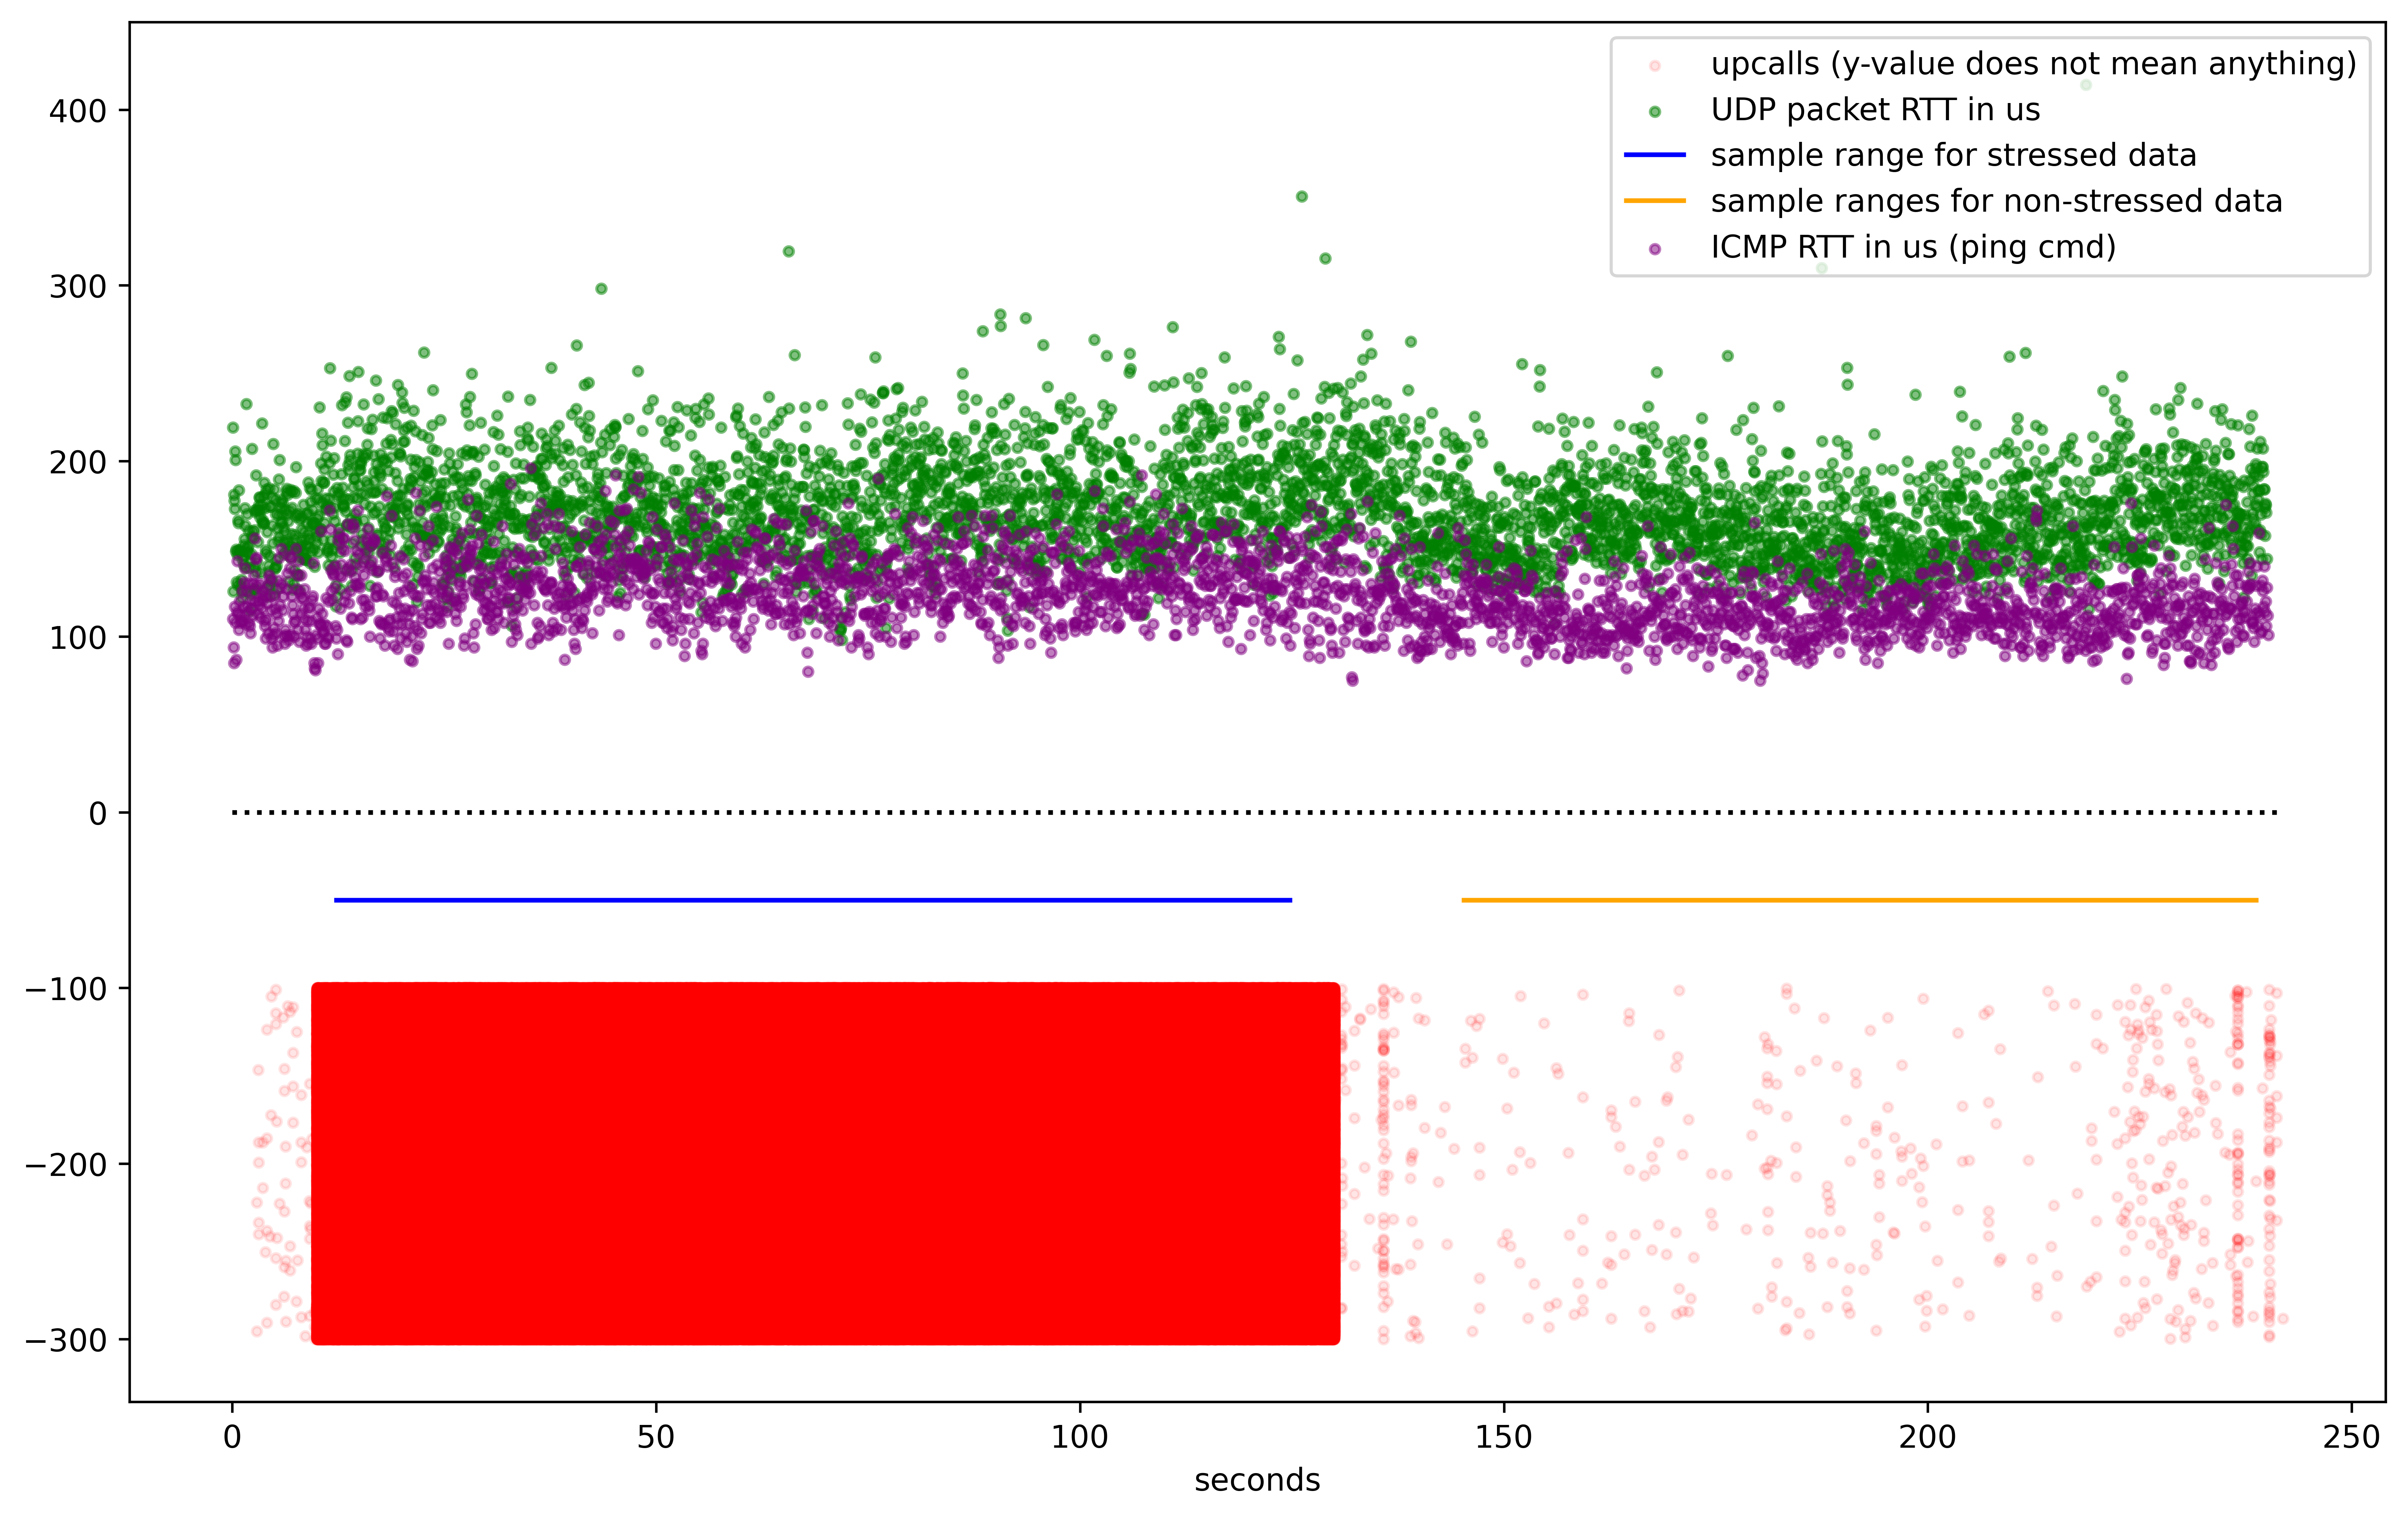
\includegraphics[width=.9\linewidth]{img/packet_flood_50k_latency.png}
    \caption{Round trip times during 50k upcalls/sec stress test}
    \label{fig:plot-packet-flood-50k-latency}
\end{figure}

\Cref{fig:plot-packet-flood-50k-latency} shows the results of a different run of the same experiment. The plot shows only the latencies measured from the \ident{victim} pod. The ICMP tests target the node IP address of \kb{1}, and the UDP tests target the \ident{reflector} service provided by a pod on \kb{3}. The horizontal lines mark the ranges of samples used for a statistical test.

While there does not seem to be any substantial difference between the stressed and non-stressed systems in the round-trip times, the non-stressed UDP samples ($n=1876$, $\bar{x}=175980 \pm 1320$ \si{\nano\second}\footnote{$95\%$ confidence interval, assuming normal distribution}) are smaller than the stressed UDP samples ($n=2255$, $\bar{x}=164404 \pm 1174$ \si{\nano\second}) with statistical significance (Welch's t-test, $p=2.17 \cdot 10^{-37}$). The difference between the means is $11576$ \si{\nano\second}.

% stressed UDP latency
% shape: (9, 3)
% ┌────────────┬────────────┬───────────────┐
% │ describe   ┆ ts         ┆ latency_ns    │
% │ ---        ┆ ---        ┆ ---           │
% │ str        ┆ f64        ┆ f64           │
% ╞════════════╪════════════╪═══════════════╡
% │ count      ┆ 2255.0     ┆ 2255.0        │
% │ null_count ┆ 0.0        ┆ 0.0           │
% │ mean       ┆ 68.502237  ┆ 175980.142794 │
% │ std        ┆ 32.628849  ┆ 31963.391742  │
% │ min        ┆ 12.025217  ┆ 98250.0       │
% │ max        ┆ 124.979466 ┆ 762959.0      │
% │ median     ┆ 68.502056  ┆ 173259.0      │
% │ 25%        ┆ 40.238689  ┆ 155156.0      │
% │ 75%        ┆ 96.765862  ┆ 193006.0      │
% └────────────┴────────────┴───────────────┘
% (175980.14279379157, 174660.18226166346, 177300.10332591968)
% non-stressed UDP latencies
% shape: (9, 3)
% ┌────────────┬────────────┬───────────────┐
% │ describe   ┆ ts         ┆ latency_ns    │
% │ ---        ┆ ---        ┆ ---           │
% │ str        ┆ f64        ┆ f64           │
% ╞════════════╪════════════╪═══════════════╡
% │ count      ┆ 1876.0     ┆ 1876.0        │
% │ null_count ┆ 0.0        ┆ 0.0           │
% │ mean       ┆ 191.99893  ┆ 164404.665245 │
% │ std        ┆ 27.143008  ┆ 25925.644717  │
% │ min        ┆ 145.023486 ┆ 107262.0      │
% │ max        ┆ 238.975234 ┆ 495776.0      │
% │ median     ┆ 191.999098 ┆ 161704.5      │
% │ 25%        ┆ 168.52374  ┆ 146410.0      │
% │ 75%        ┆ 215.52409  ┆ 178624.0      │
% └────────────┴────────────┴───────────────┘
% (164404.66524520254, 163230.7366655189, 165578.5938248862)


\subsection{Performance when resource limited}

In \cref{subsec:standard-behavior}, we talked about extra memory and CPU usage of \ident{ovs-vswitchd}. The default containerized deployment of OVN-Kubernetes \href{https://github.com/ovn-org/ovn-kubernetes/blob/b982b8cadba939c55010829f61eb5ebe4fd90794/dist/templates/ovs-node.yaml.j2#L84-L90}{limits} \ident{ovs-vswitchd} to 400 MiB of physical memory and two-tenths of a single CPU core. In the remainder of this section, when we write about limiting memory or CPU, we mean using Kubernetes to enforce the resource limit just as the default containerized deployment does it.

\subsubsection{Memory limit}
\label{subsec:memory}
We limited the memory usage of \ident{ovs-vswitchd}, leaving the CPU time unlimited. We used the default values for the memory limit, leaving us with the following configuration of the OVS container:

\begin{Verbatim}[fontsize=\small]
resources:
    requests:
        memory: 300Mi
    limits:
        memory: 400Mi
\end{Verbatim}

When we flooded the system with upcalls, \ident{ovs-vswitchd} crashed without leaving any meaningful error message behind. During normal operations, everything seemed normal.

We tried to limit the number of flow rules using the following command:
\begin{Verbatim}[fontsize=\small]
ovs-vsctl set Open_vSwitch . other_config:flow-limit=10000
\end{Verbatim}

The limit helps and when the upcall frequency is not too high (double or triple the limit), everything works. However, once we flood the network with even more packets, the flow limit is overshot and \ident{ovs-vswitchd} again crashes.

Our theory is that the crash happens during the revalidator dump phase, when \ident{ovs-vswitchd} makes a copy of all in-kernel flow rules in the userspace. This allocates more memory than allowed and the container is subsequently terminated by the OOM killer. Quoting Kubernetes Documentation \cite{KubeMemoryLimits}:

\begin{quote}
    A Container can exceed its memory request if the Node has memory available. But a Container is not allowed to use more than its memory limit. If a Container allocates more memory than its limit, the Container becomes a candidate for termination. If the Container continues to consume memory beyond its limit, the Container is terminated. If a terminated Container can be restarted, the kubelet restarts it, as with any other type of runtime failure.
\end{quote}

The decreased flow limit in the configuration of OVS does not help much to prevent crashes, because we can inject too many flows in between the revalidator thread runs (we can inject about 100k flow rules in 500ms, \ident{ovs-vswitch} crashes even with less).

\subsubsection{CPU limit}
\label{subsec:cpu-limit}

When CPU bound, \ident{ovs-vswitchd} does not crash. It tries to do the opposite and \href{https://github.com/openvswitch/ovs/blob/e3ba0be48ca457ab3a1c9f1e3522e82218eca0f9/ofproto/ofproto-dpif-upcall.c\#L1031-L1041}{dynamically changes the datapath's flow rule limit} based on the revalidator thread's performance:

\begin{Verbatim}[fontsize=\small]
duration = MAX(time_msec() - start_time, 1);
udpif->dump_duration = duration;
if (duration > 2000) {
    flow_limit /= duration / 1000;
} else if (duration > 1300) {
    flow_limit = flow_limit * 3 / 4;
} else if (duration < 1000 &&
            flow_limit < n_flows * 1000 / duration) {
    flow_limit += 1000;
}
flow_limit = MIN(ofproto_flow_limit, MAX(flow_limit, 1000));
\end{Verbatim}

We can see the effect of this code in \cref{fig:packet-flood-limited}. The red dots signify the dynamic flow limit. The horizontal lines going to the right of the dots signify the time the revalidator run took. We can see that a long revalidator run leads to a decreased flow limit.

% QT_QPA_PLATFORM=xcb python postprocessing/packet_flood.py results/packet_flood_2023-06-11T21:15+02:00/
\begin{figure}
    \centering
    \includegraphics[width=.9\linewidth]{img/packet_flood_limited_resources_50k.png}
    \caption{5k upcalls/sec stress test}
    \label{fig:packet-flood-limited}
\end{figure}

 When compared to the previous experiments:

\begin{itemize}
    \item The rate of upcalls is only $5000$ per second, one-tenth of the experiments before.
    \item Memory usage stays almost constant.
    \item Load average (1 minute) peaks at the value 2, but stays below 1 most of the time.
    \item The size of the datapath flow table varies a lot more. We can see the same higher frequency variations as before, but now they are combined with lower frequency variations created by the dynamically changing flow limit.
    \item Latency measurements are added to the plot (beware of the unusual units). The measurement method is the same as when we talked about latency before, now combined into a single experiment. The highest round-trip time observed is around 10 seconds long. Sometimes, sending a packet completely fails (indicated by thicker dots below the number line). The lines signify when the packet was in-flight.
\end{itemize}

The extremely high round-trip times can be explained by the upcall buffer queues. When the revalidator threads and other tasks use most of the available resources, the handler threads might not get scheduled and the packets in upcalls are buffered until the handler threads run again. This explains the regular packet delivery pattern (the green diagonal lines on the plot). They are caused by a regular packet-sending interval and a single instant when all the packets are delivered in one big batch.

\paragraph{Flood with 200k packets per second}
When we send 200k packets per second (close to the limit of our tool's single-threaded performance), \ident{ovs-vswichd} does not crash, but no network traffic is getting through. The \ident{victim} pod on the same host was unable to receive any packet.

Interestingly, when we stop the stress test, the number of flow rules still oscillates for a couple of seconds before dropping to normal levels. This indicates that our hypothesis about queues in front of the handler threads was correct and that there are a lot of packets queued for processing. 

\subsubsection{CPU and memory limit}

When we use the default configuration with both CPU and memory limits, \ident{ovs-vswitchd} is still killed by OOM killer under extreme stress (200k upcall generating packets per second), even though the memory usage stays below the limit most of the time. The crashes are however not reliable and sometimes, \ident{ovs-vswitchd} runs normally for a while. The problem seems to be caused by a race condition between the flow limit calculation in revalidator threads and the handler threads inserting new flow rules. The crash happens when we change something - either at the beginning of a stress test or at the end, regardless of how long it is.

\subsection{Overloading \ident{ovs-vswitchd} without resource limits}

The crashes of \ident{ovs-vswitchd} led us to search for a possibility of a crash when overloaded without resource constraints. We tried to spawn multiple instances of our packet flooding tool, intentionally more threads than we had CPU cores available. On the 28-core dedicated test servers, we did not manage to crash \ident{ovs-vswitchd} with anywhere between 1 and 80 instances of our stress tool.

We believe that \ident{ovs-vswitchd} is safe from crashes as long as it runs without resource constraints. On our experimental clusters, \ident{ovs-vswitchd} is automatically configured as a higher priority process than the ordinary processes and therefore it gets enough CPU time. But even if we manually decrease the priority to the same level or below ordinary processes, \ident{ovs-vswitchd} does not crash.
